\documentclass[a1paper,landscape,25pt]{tikzposter}

\usepackage{amsmath}
\usepackage{pgf,tikz,pgfplots}
\pgfplotsset{compat=1.15}
\usepackage{mathrsfs}
\usetikzlibrary{arrows}


\settitle{
  \vspace{-5cm}
  \centering \vbox{
\@titlegraphic \\[\TP@titlegraphictotitledistance] \centering
\color{titlefgcolor} {\bfseries \fontsize{90}{100} \sc \@title \par}
\vspace{0em}
}}

\title{Rechten}

\addtolength{\jot}{1em}

\usetheme{Basic}
\usecolorstyle[colorOne=teal,colorTwo=cyan,colorThree=gray]{Spain}

\tikzposterlatexaffectionproofoff

\definenotestyle{notestyle}{
  targetoffsetx=0pt, targetoffsety=0pt, angle=90, radius=3cm,
  width=6cm, connection=false, rotate=0, roundedcorners=20, linewidth=1pt,
  innersep=1cm
}{
  \ifNoteHasConnection
  \draw[thick] (notecenter) -- (notetarget) node{$\bullet$};
  \fi
  \draw[draw=notebgcolor,fill=notebgcolor,rotate=\noterotate,rounded corners=\noteroundedcorners]
  (notecenter.south west) rectangle (notecenter.north east);
}
\usenotestyle{notestyle}

\begin{document}

\maketitle

\begin{columns}
  \column{0.75}
  \block{Grafisch}{
    \begin{center}
      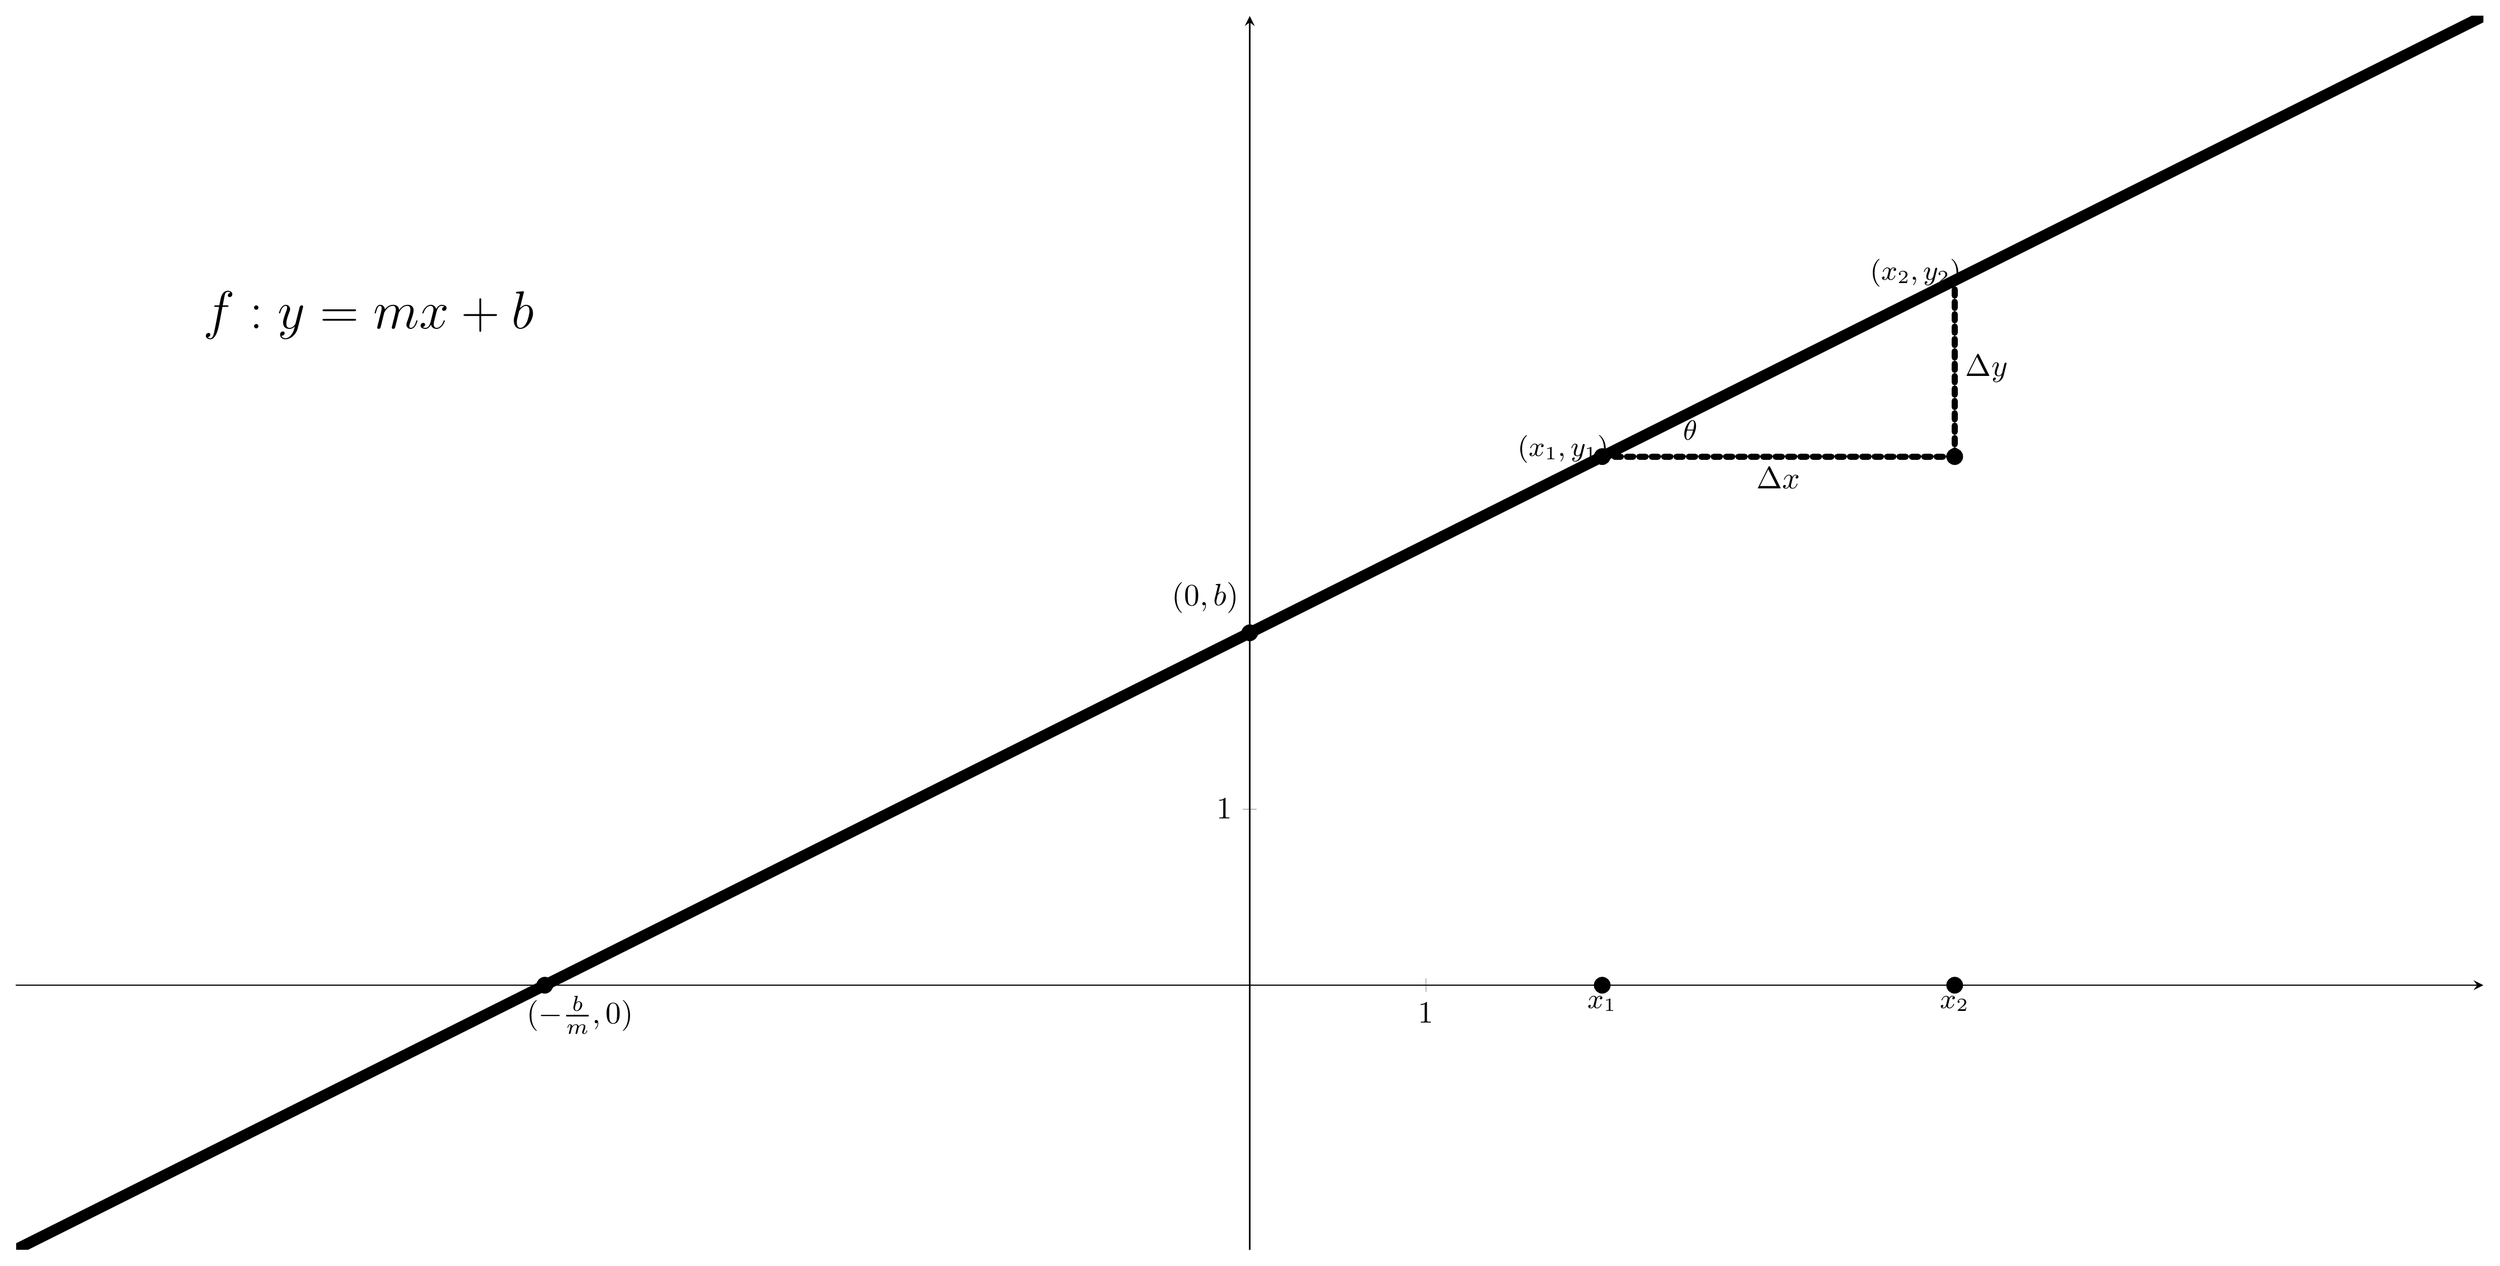
\begin{tikzpicture}[scale=2,line cap=round,line join=round,>=triangle 45,x=1.0cm,y=1.0cm]
        \begin{axis}[
          x=2.0cm,y=2.0cm,
          axis lines=middle,
          xmin=-7, xmax=7, ymin=-1.5, ymax=5.5,
          xtick={0,1}, ytick={0,1}
          ]
          \clip(-7,-1.5) rectangle (7,5.5);
          \draw [line width=3.6pt,domain=-7:7]
          plot(\x,{(--4--\x)/2});
          \draw [line width=2.pt,dotted] (2,3)-- (4,3);
          \draw [line width=2.pt,dotted] (4,3)-- (4,4);
          \draw (-3.8,0) node[anchor=north] {$(-\frac{b}{m},0)$};
          \draw (0,2.2) node[anchor=east] {$(0,b)$};
          \draw (2.1,2.9) node[anchor=south east] {\small$(x_1,y_1)$};
          \draw (4.1,3.9) node[anchor=south east] {\small $(x_2,y_2)$};
          \draw (3,3) node[anchor=north] {$\Delta x$};
          \draw (4,3.5) node[anchor=west] {$\Delta y$};
          \draw (2.4,3.15) node[anchor=west] {\small $\theta$};
          \draw (-6,4) node[anchor=north west] {\LARGE $f: y=mx+b$};
          \draw [fill=black] (-4,0) circle (2.5pt);
          \draw [fill=black] (0,2) circle (2.5pt);
          \draw [fill=black] (2,3) circle (2.5pt);
          \draw [fill=black] (4,3) circle (2.5pt);

          \draw [fill=black] (2,0) circle (2.5pt);
          \draw [fill=black] (4,0) circle (2.5pt);
          \draw (2,0) node[anchor=north] {\small$x_1$};
          \draw (4,0) node[anchor=north] {\small $x_2$};
        \end{axis}
      \end{tikzpicture}
    \end{center}
  }
  \column{0.25}
  \block{Rico}{
    \LARGE
    \begin{align*}
      m &= \dfrac{y_2-y_1}{x_2-x_1}
    \end{align*}
  }
  \block{Differentiequotiënt}{
    \LARGE
    \begin{align*}
      \dfrac{\Delta y}{\Delta x}_{[x_1,x_2]} &= \dfrac{f(x_2)-f(x_1)}{x_2-x_1}
    \end{align*}
  }
  \block{Hellingshoek $\theta$}{
    \LARGE
    \begin{align*}
      \tan \theta &= \dfrac{\Delta y}{\Delta x}
    \end{align*}
  }
\end{columns}

  \begin{columns}
    \column{0.4}
    \block{Rico $m$ en één punt $(x_1,y_1)$}{
      \LARGE
      \begin{align*}
        y - y_1 &= m(x - x_1)
      \end{align*}
    }
    \block{Punten $(x_1,y_1)$ en $(x_2, y_2)$}{
      \LARGE
      \begin{align*}
        y - y_1 &= \dfrac{y_2-y_1}{x_2-x_1}(x - x_1)
      \end{align*}
    }
    \column{0.6}
    \block{Rechten in de ruimte}{
      \LARGE
      \begin{minipage}{.5\linewidth}
        \innerblock{Parametervergelijking}{
          $$\begin{cases}
            x &= x_0 + ka\\
            y &= y_0 + kb\\
            z &= z_0 + kc
          \end{cases}$$
        }
      \end{minipage}
      \begin{minipage}{.5\linewidth}
        \innerblock{Cartesische vergelijking}{
          $$\dfrac{x-x_0}{a}=\dfrac{y-y_0}{b}=\dfrac{z-z_0}{c}$$
        }
      \end{minipage}
    }
  \end{columns}

\end{document}
